% -*- coding: UTF-8; -*-
\documentclass[11pt]{article}

\usepackage[utf8]{inputenc}
\usepackage[english]{babel}

\usepackage[top=2cm, bottom=2cm, left=2cm, right=2cm, columnsep=20pt]{geometry}  
\usepackage{graphicx}      
\usepackage{url}           
\usepackage{verbatim}      
\usepackage{amsmath}
\usepackage{cancel}
\usepackage[usenames]{color}
\usepackage{mathrsfs}
\usepackage{amssymb}
\usepackage{mathtools}
\usepackage{xfrac}
\usepackage{float}
\usepackage{wrapfig}
\usepackage{framed}
\usepackage{subcaption}
\usepackage{listings}
\usepackage{siunitx}
\usepackage[linesnumbered,ruled]{algorithm2e}
\usepackage{algorithmicx}
\allowdisplaybreaks

\begin{document}

\begin{titlepage} % Suppresses displaying the page number on the title page and the subsequent page counts as page 1
	\newcommand{\HRule}{\rule{\linewidth}{0.5mm}} % Defines a new command for horizontal lines, change thickness here
	
	\center % Centre everything on the page
	\vspace*{2cm}
	
	%------------------------------------------------
	%	Headings
	%------------------------------------------------
	
	\textsc{\LARGE Universit\'e de Montr\'eal}\\[1cm] % Main heading such as the name of your university/college
	\textsc{\Large IFT6269 - Probabilistic Graphical Models}\\[2cm] % Major heading such as course name
		
	%------------------------------------------------
	%	Title
	%------------------------------------------------
	
	\HRule\\[0.5cm]
	{\huge\bfseries Homework 4}\\[0.2cm] % Title of your document
	\HRule\\[3cm]
	
	%------------------------------------------------
	%	Author(s)
	%------------------------------------------------
	
	{\large\textit{Author}}\\
	 Patrice \textsc{B\'echard}\\ % Your name
	 20019173
	
	%------------------------------------------------
	%	Date
	%------------------------------------------------
	
	\vfill\vfill\vfill % Position the date 3/4 down the remaining page
	
	{\large\today} % Date, change the \today to a set date if you want to be precise
	
	%------------------------------------------------
	%	Logo
	%------------------------------------------------
	
	%\vfill\vfill
	%
\includegraphics[width=0.2\textwidth]{~/placeholder.jpg}\\[1cm] % Include a department/university logo - this will require the graphicx package
	 
	%----------------------------------------------------------------------------------------
	
	\vfill % Push the date up 1/4 of the remaining page
	
\end{titlepage}

\section{Entropy \& Mutual Information}\label{sec:num1}

\begin{enumerate}

\item Let $X$ be a discrete random variable on a finite space $\mathcal{X}$ with $|\mathcal{X}| = k$.

	\begin{description}
	
	\item[(a)] We know that the entropy is given by :
	
		\begin{align}
			H(X) & \triangleq -\sum_{x \in \mathcal{X}} p(x) \log p(x) \\
				 & = - \sum_{i = 1}^{k} p(X=x_i) \log p(X=x_i) \nonumber
		\end{align}
		
		where we sum over all possible values that $X$ can take. In the general case, where $X$ can take multiple possible values, knowing that the probability $p(X=x_i)$ of an event happening is $\in [0,1[$ and knowing that the logarithm of a value in that range is always negative, we have:
		
		\begin{align*}
			H(X) & = - \sum_{i = 1}^{k} \underbrace{p(X=x_i)}_{\in [0,1[} \underbrace{\log p(X=x_i)}_{\text{always } <0}
		\end{align*}
		
		We thus have \textbf{minus} the sum of $k$ \textbf{negative} terms, which yields a \textbf{positive} value. However, if $X$ is a constant, then $p(X=x) = 1$ and $\log p(X=x) = 0$. In that case, the entropy is given by :
		
		\begin{align*}
			H(X) = - \underbrace{p(X=x)}_{1} \underbrace{\log p(X=x)}_{0} = 0
		\end{align*}
		
		We thus have proven that $H(x) \geq 0$, with equality only when $X$ is a constant. $\blacksquare$

%]]]] just to close brackets a bit higher
	
	\item[(b)] We now denote by $p$ the distribution of $X$ and $q$ the uniform distribution on $\mathcal{X}$. We know that the Kullback-Leibler divergence is given by :
	
		\begin{align}
			D_{KL}(p||q) & \triangleq \sum_{x \in \mathcal{X}} p(x) \log \frac{p(x)}{q(x)}
		\end{align}
		
		We can develop this expression :
		
		\begin{align}\label{eq:kl_entropy}
			D_{KL}(p||q) & = \underbrace{\sum_{x\in \mathcal{X}} p(x) \log p(x)}_{-H(X)} - \sum_{x \in \mathcal{X}} p(x) \log \underbrace{q(x)}_{=1/k} \nonumber \\
						 & = -H(X) - \left(\log \frac{1}{k}\right) \underbrace{\sum_{x \in \mathcal{X}} p(x)}_{1} \nonumber \\
						 & = -H(X) + \log k
		\end{align}
		
		We find that the Kullback-Leibler divergence $D_{KL}(p||q)$ is simply minus the entropy $H(X)$ of the distribution $p$ plus the logarithm of the number of possible values that $X$ can take.
	
	\item[(c)] Knowing that maximizing entropy is the same as minimizing the Kullback-Leibler divergence, and knowing that one of the properties of the Kullback-Leibler divergence is that $D_{KL}(p||q) \geq 0$, we can use the result obtained in the previous problem (equation \ref{eq:kl_entropy}) to find an upper bound on the entropy that depends on $k$:
	
		\begin{align*}
			D_{KL}(p||q) & = -H(X) + \log k \\
			H_{max}(X) & = \log k - \underbrace{D_{KL, min}(p||q)}_{0} \\
			\Aboxed{H_{max}(X) & = \log k}
		\end{align*}
		
	
	\end{description}


\item Considering a pair of random variables $(X_1, X_2)$ defined over the finite set $\mathcal{X}_1 \times \mathcal{X}_2$. Let $p_{1,2}$, $p_1$ and $p_2$ denote respectively the joint distribution, the marginal distribution of $X_1$ and the marginal distribution of $X_2$. The mutual information $I(X_1, X_2)$ is defined as :

\begin{equation}\label{eq:mutual_info}
I(X_1, X_2) := \sum_{(x_1,x_2) \in \mathcal{X}_1 \times \mathcal{X}_2} p_{1,2}(x_1, x_2) \log \frac{p_{1,2}(x_1,x_2)}{p_1(x_1)p_2(x_2)}
\end{equation}

	\begin{description}
	
	\item[(a)] We can prove that $I(X_1,X_2) \geq 0$. First, we notice that $\sum_{(x_1,x_2)\in \mathcal{X}_1,\mathcal{X}_2} p_{1,2}(x_1,x_2) = 1$. Second, we see that by inverting the logarithm, we can obtain a convex function :
	
	\begin{align*}
		I(X_1,X_2) = - \sum_{(x_1,x_2)\in \mathcal{X}_1,\mathcal{X}_2} p_{1,2}(x_1,x_2) \log \frac{p_1(x_1)p_2(x_2)}{p_{1,2}(x_1,x_2)}
	\end{align*}
	
	We can apply Jensen's inequality on the convex function to obtain :
	
	\begin{align*}
	I(X_1,X_2) & \geq -\log \left[ \sum_{(x_1,x_2)\in \mathcal{X}_1,\mathcal{X}_2} \cancel{p_{1,2}(x_1,x_2)}\frac{p_1(x_1)p_2(x_2)}{\cancel{p_{1,2}(x_1,x_2)}} \right]\\
			   & = -\log \left[ \sum_{(x_1,x_2)\in \mathcal{X}_1,\mathcal{X}_2}p_1(x_1)p_2(x_2) \right] \\
			   & = 0\qquad \blacksquare
	\end{align*}
	
	\item[(b)] By starting from the definition of the mutual information (equation \ref{eq:mutual_info}), writing the sum over all possible states $\sum_{(x_1,x_2) \in \mathcal{X}_1 \times \mathcal{X}_2}$ as $\sum_{x_1, x_2}$, we have :
	
		\begin{align*}
		I(X_1, X_2) & = \sum_{x_1,x_2} p_{1,2}(x_1, x_2) \log \frac{p_{1,2}(x_1,x_2)}{p_1(x_1)p_2(x_2)} \\
					& = \underbrace{\sum_{x_1,x_2} p_{1,2}(x_1, x_2) \log p_{1,2} (x_1, x_2)}_{-H(X_1,X_2)} - \sum_{x_1,x_2} p_{1,2}(x_1,x_2) \log p(x_1) - \sum_{x_1,x_2} p_{1,2}(x_1,x_2) \log p(x_2) \\
					& = - H(X_1,X_2) - \sum_{x_1,x_2} p(x_2\mid x_1) p(x_1) \log p(x_1) - \sum_{x_1,x_2} p(x_1\mid x_2) p(x_2) \log p(x_2) \\
					& = - H(X_1,X_2) - \sum_{x_1} \left( p(x_1)\log p(x_1) \underbrace{\sum_{x_2} p(x_2\mid x_1)}_{=1}\right) - \sum_{x_2} \left( p(x_2)\log p(x_2) \underbrace{\sum_{x_1} p(x_1\mid x_2)}_{=1} \right) \\
					& = -H(X_1,X_2) - \underbrace{\sum_{x_1} p(x_1) \log p(x_1)}_{-H(X_1)} - \underbrace{\sum_{x_2} p(x_2) \log p(x_2)}_{-H(X_2)} \\
					& = -H(X_1,X_2) + H(X_1) + H(X_2)
		\end{align*}
	
	\item[(c)] Since the mutual information $I(X_1,X_2) \geq 0$, we have that the maximum entropy that $p_{1,2}(x_1,x_2)$ can have is $H_{\mathrm{max}}(X_1,X_2) = H(X_1) + H(X_2)$. This happens when $p_{1,2}(x_1,x_2) = p_1(x_1)p_2(x_2)$, that is when random variables $X_1$ and $X_2$ are mutually independent.
	
	\end{description}


\end{enumerate}


\section{HMM - Implementation}\label{sec:num2}

\begin{enumerate}

\item The implementation of the $\alpha$ and $\beta$ recursions can be found in the file \texttt{hwk4.ipynb}. They are implemented as the methods \texttt{\_forward} and \texttt{\_backward} of the \texttt{HMM} class. This is a great example of dynamic programming, where we initiate an empty array of $\alpha$ or $\beta$ values, we first compute the base case for both cases, and we continue to compute the following values using the values already in the array. We will be able to compute the \textit{smoothing} distribution $\gamma_{t} ^{(i)} = p\left(z_{t} ^{(i)}|\mathbf{x},\theta\right)$ and the pair-marginals $\xi_{t-1,t} ^{(i,j)} = p\left(z_{t-1} ^{(i)}, z_{t} ^{(j)}|\mathbf{x}, \theta \right)$. We can develop to find these distributions as functions of $\alpha$ and $\beta$ :

\begin{align*}
\gamma_t ^{(i)} & = p\!\left(z_{t} ^{(i)}|\mathbf{x}\right)\\
				& = \frac{p\!\left(\mathbf{x}|z_{t} ^{(i)}\right) p\!\left(z_{t} ^{(i)}\right)}{p(\mathbf{x})} \\
				& = \frac{p\!\left(x_{1},\dots,x_{t}|z_{t} ^{(i)}\right) p\!\left( x_{t+1},\dots,x_{T} |z_{t} ^{(i)} \right) p\!\left(z_{t} ^{(i)}\right)}{p(\mathbf{x})}\\
				& = \frac{\alpha_t ^{(i)} \beta_t ^{(i)}}{\sum_{k=1}^{K} \alpha_t ^{(k)} \beta_t ^{(k)}}
\end{align*}

\begin{align*}
\xi_{t-1, t} ^{(i,j)} & = p\!\left(z_{t-1} ^{(i)}, z_{t} ^{(j)}|\mathbf{x}\right) \\
					  & = \frac{p\!\left(\mathbf{x}|z_{t-1}^{(i)},z_{t} ^{(j)}\right) p\!\left(z_{t-1}^{(i)},z_{t}^{(j)}\right)}{p(\mathbf{x})} \\
					  & = \frac{p\!\left(x_1,\dots, x_{t-1}|z_{t-1}^{(i)}\right) p\!\left(x_{t}|z_{t}^{(j)}\right) p\!\left( x_{t+1},\dots,x_{T}|z_{t}^{(j)} \right) p\!\left(z_{t}^{(j)}|z_{t-1}^{(i)}\right) p\!\left(z_{t-1}^{(i)}\right)}{p(\mathbf{x})} \\
					  & = \frac{\alpha_{t-1}^{(i)} \; \mathcal{N}\!\!\left( x_t | \mu_j, \Sigma_j  \right) A_{ji} \;\beta_{t}^{(i)}}{p(\mathbf{x})}
\end{align*}

\item Using the same parameters for the means and covariance matrix of the 4 Gaussians learned in homework 3 (these are given here), and initializing the initial probability distribution $\pi_k = \frac{1}{4}$ and setting $A$ to be the matrix with diagonal coefficients $A_{ii}=\frac{1}{2}$ and off-diagonal coefficients $A_{ij} = \frac{1}{6}$ for all $(i,j) \in \{1 \dots 4\}^2$, we can compute the $\alpha_t$'s and $\beta_t$'s using the implementation of the $\alpha$ and $\beta$ recursions. We can compute the smoothing distribution $\gamma_t ^{(i)}$. Figure \ref{fig:prob_alphabeta} presents the probability for each of the 4 states as a function of $t$ for the first 100 datapoints in the file \texttt{EMGaussian.test}.

\begin{figure}[htbp]
\begin{center}
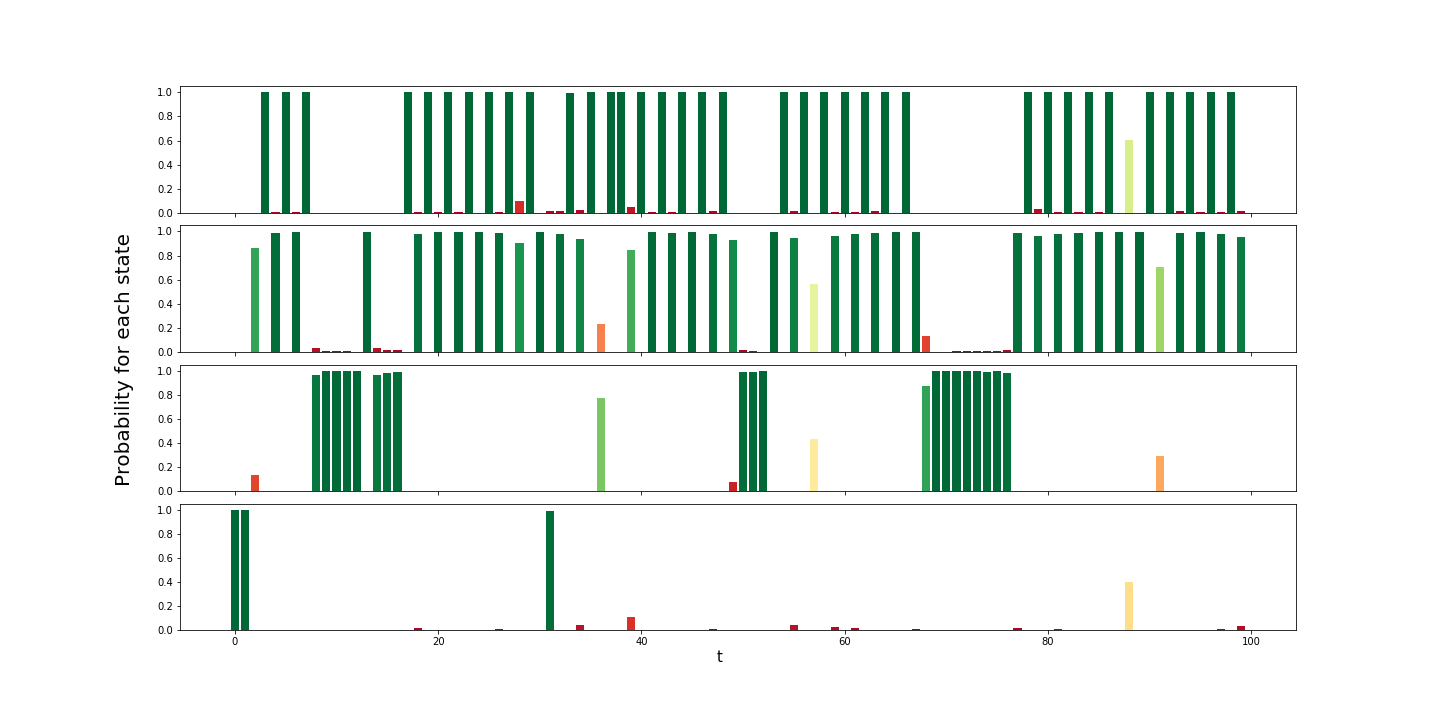
\includegraphics[width=\textwidth]{figures/fake_param_inference.png}
\caption{Probability $p(z_t\mid x_1,\dots , x_T)$ for each of the 4 states (top panel is state 1, bottom panel is state 4) as a function of $t$ for the first 100 datapoints in the file \texttt{EMGaussian.test}. The color of each bar represents the probability of the datapoint for each state, going from red to green}
\label{fig:prob_alphabeta}
\end{center}
\end{figure}

\item Here we derive the M-step update for $\hat{\pi}$, $\hat{A}$, $\hat{\mu}_k$ and $\hat{\Sigma}_k$ for $k=1, \dots, 4$ during the EM algorithm, as a function of the quantities computed during the E-step. We first start by taking the log-likelihood of the probability distribution given by the HMM :


\begin{align*}
\log p(x,z|\theta) & = \log \left( p(z_1 | \pi) \prod_{t=2}^{T} p(z_t|z_{t-1},A) \prod_{t=1}^{T} p(x_t|z_t,\mu,\Sigma) \right) \\
				   & = \log \left( \prod_{k=1}^{K} \pi_{k} ^{z_{1}^{(k)}} \prod_{t=2}^{T} \prod_{i=1}^{K} \prod_{j=1}^{K} A_{ji}^{z_{t-1}^{(i)}z_{t}^{(j)}} \prod_{t=1}^{T} \prod_{k=1}^{K} \mathcal{N}(x_t|\mu_k,\Sigma_k)^{z_{t}^{(k)}} \right) \\
				   & = \sum_{k=1}^{K} z_{1}^{(k)} \log \pi_{k} + \sum_{t=2}^{T} \sum_{i=1}^{K}\sum_{j = 1}^{K} \left[z_{t-1}^{(i)}z_{t}^{(j)} \right] \log A_{ji} + \sum_{t=1}^{T} \sum_{k=1}^{K} z_{t}^{(k)} \log\mathcal{N}(x_t|\mu_k,\Sigma_k)\\
				   & = \sum_{k=1}^{K} \gamma_{1}^{(k)} \log \pi^{k} + \sum_{t=2}^{T} \sum_{i=1}^{K}\sum_{j = 1}^{K} \xi_{t-1,t}^{(i,j)} \log A_{ji} + \sum_{t=1}^{T} \sum_{k=1}^{K} \gamma_{t}^{(k)} \log\mathcal{N}(x_t|\mu_k,\Sigma_k)\\
\end{align*}


where we have substituted for the appropriated sufficient statistics. Now, all that we have to do is to derivate with respect to the wanted parameter to find the wanted update. Starting with $\pi^{(k)}$, we have, using the constraint that $\sum_{k=1}^{K} \pi_k = 1$ and using the Lagrange multipliers method:

{\small
\begin{align*}
\frac{\partial}{\partial \pi_k} \log p(x,z|\theta) & = \frac{\partial}{\partial \pi_k}\left[ \sum_{k=1}^{K} \gamma_{1}^{(k)} \log \pi_{k} + \cancel{\sum_{t=2}^{T} \sum_{i=1}^{K}\sum_{j = 1}^{K} \xi_{t-1,t}^{(i,j)} \log A_{ji}} + \cancel{\sum_{t=1}^{T} \sum_{k=1}^{K} \gamma_{t}^{(k)} \log\mathcal{N}(x_t|\mu_k,\Sigma_k)} - \lambda\left(\sum_{k=1}^{K} \pi_k - 1\right)\right]\\
												   & = \frac{\partial}{\partial \pi_k} \left[\sum_{k=1}^{K} \gamma_{1}^{(k)} \log \pi_{k} - \lambda\left(\sum_{k=1}^{K} \pi_{k} - 1\right)\right]\\
												   & =	\frac{\gamma_{1}^{(k)}}{\pi_k} - \lambda \\
												   & = 0 \\
\end{align*}
We then have :
\begin{align*}
								\frac{\gamma_{1}^{(k)}}{\pi_k} &= \lambda \\
								\pi_k &= \frac{\gamma_{1}^{(k)}}{\lambda}	   
\end{align*}
}

Using the constraint, we find that $\lambda = \sum_{i=1}^{K} \gamma_{1}^{(k)}$, which gives us :

\begin{align*}
\boxed{\hat{\pi}_k = \frac{\gamma_{1}^{(k)}}{\sum_{i=1}^{K} \gamma_{1}^{(k)}}}
\end{align*}

We now do the same with the transition matrix to find the update of $A_{ij}$, using the Lagrange multipliers method and the constraint that $\sum_{i=1}^{K} A_{ij} = 1$ :

{\small
\begin{align*}
\frac{\partial}{\partial A_{ij}} \log p(x,z|\theta) & = \frac{\partial}{\partial A_{ij}}\left[ \cancel{\sum_{k=1}^{K} \gamma_{1}^{(k)} \log \pi_{k}} + \sum_{t=2}^{T} \sum_{i=1}^{K}\sum_{j = 1}^{K} \xi_{t-1,t}^{(i,j)} \log A_{ji} + \cancel{\sum_{t=1}^{T} \sum_{k=1}^{K} \gamma_{t}^{(k)} \log \mathcal{N}(x_t|\mu_k,\Sigma_k)} - \lambda\left(\sum_{i=1}^{K} A_{ij} - 1\right)\right]\\
													& = \frac{\partial}{\partial A_{ij}} \left[ \sum_{t=2}^{T} \sum_{i=1}^{K}\sum_{j = 1}^{K} \xi_{t-1,t}^{(i,j)} \log A_{ji} - \lambda\left(\sum_{i=1}^{K} A_{ij} - 1\right)\right]\\
													& = \frac{\sum_{t=2}^T \xi_{t-1,t}^{(i,j)}}{A_{ij}} - \lambda \\
													& = 0
\end{align*}
We then have :
\begin{align*}
\frac{\sum_{t=2}^{T} \xi_{t-1,t}^{(i,j)}}{A_{ij}} & = \lambda \\
A_{i,j} &= \frac{\sum_{t=2}^T \xi_{t-1,t}^{(i,j)}}{\lambda}
\end{align*}
}

Once again, using the constraint that each column of the transition matrix must sum to 1, we find :

\begin{align*}
\boxed{\hat{A}_{ij} = \frac{\sum_{t=2}^{T}\xi_{t-1,t}^{(i,j)}}{\sum_{l=1}^{K} \sum_{t=2}^{T} \xi_{t-1,t}^{(i,l)}}}
\end{align*}

We now do the same thing for both parameters $\mu$ and $\Sigma$. In this case, no need to use the Lagrange multipliers method. We will also reuse some results already found in other homework to go faster :

\begin{align*}
\frac{\partial}{\partial \mu_k} \log p(x,z|\theta) & = \frac{\partial}{\partial \mu_k}\left[ \cancel{\sum_{k=1}^{K} \gamma_{1}^{(k)} \log \pi_{k}} + \cancel{\sum_{t=2}^{T} \sum_{i=1}^{K}\sum_{j = 1}^{K} \xi_{t-1,t}^{(i,j)} \log A_{ji}} + \sum_{t=1}^{T} \sum_{k=1}^{K} \gamma_{t}^{(k)} \log\mathcal{N}(x_t|\mu_k,\Sigma_k) \right]\\
												   & = \frac{\partial}{\partial \mu_k}\left[ \sum_{t=1}^{T} \sum_{k=1}^{K} \gamma_{t}^{(k)} \log\mathcal{N}(x_t|\mu_k,\Sigma_k) \right]\\
												   & = \sum_{t=1}^{T} \gamma_{t}^{(k)} \underbrace{\frac{\partial}{\partial \mu_k} \log \mathcal{N}(x_t|\mu_k,\Sigma_k)}_{\Sigma^{-1}(x_t - \mu_k)}\\
												   & = 0
\end{align*}

We then have :

\begin{align*}
\cancel{\Sigma^{-1}} \left(\sum_{t=1}^T \gamma_{t}^{(k)} x_t - \mu_k \sum_{t=1}^T \gamma_{t}^{(k)} \right) & = 0 \\
\mu_k \sum_{t=1}^T \gamma_{t}^{(k)} & = \sum_{t=1}^T \gamma_{t}^{(k)} x_t \\
\Aboxed{\hat{\mu}_k &= \frac{\sum_{t=1}^T \gamma_{t}^{(k)} x_t}{\sum_{t=1}^T \gamma_{t}^{(k)}}}
\end{align*}

Finally, for the covariance matrix $\Sigma$, we have :

\begin{align*}
\frac{\partial}{\partial \Sigma_{k}} \log p(x,z|\theta) & = \frac{\partial}{\partial \Sigma_k}\left[ \cancel{\sum_{k=1}^{K} \gamma_{1}^{(k)} \log \pi_{k}} + \cancel{\sum_{t=2}^{T} \sum_{i=1}^{K}\sum_{j = 1}^{K} \xi_{t-1,t}^{(i,j)} \log A_{ji}} + \sum_{t=1}^{T} \sum_{k=1}^{K} \gamma_{t}^{(k)} \log\mathcal{N}(x_t|\mu_k,\Sigma_k) \right]\\
												   & = \frac{\partial}{\partial \Sigma_k}\left[ \sum_{t=1}^{T} \sum_{k=1}^{K} \gamma_{t}^{(k)} \log\mathcal{N}(x_t|\mu_k,\Sigma_k) \right]\\
												   & = \sum_{t=1}^{T} \gamma_{t}^{(k)} \underbrace{\frac{\partial}{\partial \Sigma_k} \log \mathcal{N}(x_t|\mu_k,\Sigma_k)}_{(x_t-\mu_k)(x_t-\mu_k)^T - \Sigma_k}\\
												   & = 0
\end{align*}

We finally have :

\begin{align*}
\sum_{t=1}^{T} \gamma_{t} ^{(k)} (x_t-\mu_k)(x_t-\mu_k)^T & = \Sigma_k \sum_{t=1}^T \gamma_t ^{(k)} \\
\Aboxed{\hat{\Sigma}_k & = \frac{\sum_{t=1}^{T} \gamma_{t} ^{(k)} (x_t-\mu_k)(x_t-\mu_k)^T}{\sum_{t=1}^T \gamma_t ^{(k)}}}
\end{align*}

\item %4
The implementation of the EM algorithm to learn the parameters of the model can be found in the file \texttt{hwk4.ipynb}. It is implemented in the methods \texttt{\_e\_step} and \texttt{\_m\_step} of the \texttt{HMM} class. We use the method \texttt{train} to call the EM algorithm a certain number of iterations.

\item %5
Figure \ref{fig:log_likelihood_hmm} presents the normalized log-likelihood as a function of the iterations of the algorithm for both the training set \texttt{EMGaussian.train} and the test set \texttt{EMGaussian.test}.

\begin{figure}[htbp]
\begin{center}
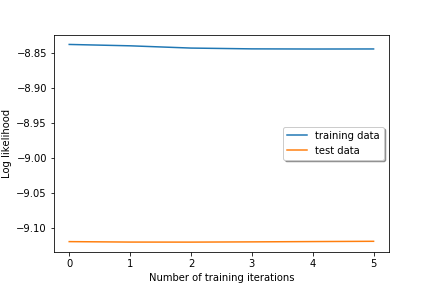
\includegraphics[width=0.6\textwidth]{figures/log_likelihood_hmm.png}
\caption{Log-likelihood as a function of the iterations of the EM algorithm for both the training set and the test set during the training of the Hidden Markov Model.}
\label{fig:log_likelihood_hmm}
\end{center}
\end{figure}

We see that the log-likelihood for both the training set and the test set remain pretty constant during the training of the HMM, which only takes 5 iterations before it converges (criteria defined by a difference of less than $0.00001$ for consecutive log-likelihood computations). We also see that the values obtained for both the training set and test set are pretty similar, even though the figure makes it look like they are really different.


\item %6
Table \ref{tab:log_likelihood} presents the values of the log-likelihoods of the full covariance Gaussian mixture model, the Gaussian mixture model with isotropic covariance matrix, the HMM and the k-means algorithm on the train and test data.

\begin{table}[htbp]
\caption{Values of the log-likelihoods for every studied model after training on the training data as well as the test data.}
\begin{center}
\begin{tabular}{l | S S }
& {Training data} & {Test data} \\
\hline

HMM & -8.84e+00 & -9.12e+00 \\
GMM (Full) & 8.65e-02 & -7.88e-02 \\
GMM (Isotropic) & -7.95e-01 & -9.05e-01 \\
K-Means & 6.70e+00 & 6.51e+00
\end{tabular}
\end{center}
\label{tab:log_likelihood}
\end{table}%

We see that the values of the normalized log-likelihoods for every model is pretty similar when comparing the value obtained with the training set and the test set. However, the values obtained for the full GMM and the HMM are pretty different from one another. This is due to the fact that the log-likelihood for both models are not computed using the same formula, which makes the comparison between these values useless. However, it can be useful to compare both GMM for different covariance matrices, since the log-likelihood is computed in the same way for both. I have included the value of the normalized objective function for the K-Means algorithm even though this is not a log-likelihood. Finally, it is not really useful to compare log-likelihood values for different models that use a different formula for log-likelihood.


\item %7

The Viterbi algorithm estimates the most likely sequence of states for a Hidden Markov Model. After having trained the model, we first select a starting state depending on the initial probability $\pi$ of each state and the emission term associated with this state. After that, for each state, we compute the most probable transition knowing the transition matrix we learned during the training process as well as the probability of each state for the last iteration. The new probabilities are the product of this probability with the emission term for this data point. After propagating this algorithm over all the data points, we propagate back to search for each most probable state starting from the end to find the most likely sequence. Algorithm \ref{alg:pseudo_viterbi} presents a pseudocode for the viterbi algorithm.

\begin{algorithm}
    \caption{Viterbi Algorithm}
    \label{alg:pseudo_viterbi}
   	\SetKwProg{Fn}{Function}{}{}
	\SetKwFunction{Viterbi}{Viterbi}%
	\Fn{\Viterbi{$x, \pi, A, T, K$}}{
	
		$\text{path} = \text{zeros}(T,K)$\;
		$\text{scores} = \text{zeros}(T,K)$\;
		\tcc{Forward propagation}
		\For(\tcc*[r]{for each data point}){$t=0$ \KwTo $T$}{
			\For(\tcc*[r]{for each state}){$k=0$ \KwTo $K$}{
				\eIf(\tcc*[r]{Base case}){$t=0$}{
					$\text{scores}[t,k] = \pi[k] * \text{emission}[x[t],k]$\;
				}{
					$\text{max\_prob\_transit} = \max(\text{scores}[t-1,k] * A[k,:])$\;
					$\text{path}[t,k] = \text{argmax}(\text{scores}[t-1,k] * A[k,:])$\;
					$\text{scores}[t,k] = \text{max\_prob\_transit} * \text{emission}[x[t],k]$\;
				}

			}
		}
		\tcc{Backward propagation}
		$\text{sequence} = \text{zeros}[t]$\;
		\For{$t=T$ \KwTo $0$}{
			\eIf(\tcc*[r]{Base case}){$t=T$}{
				$\text{sequence}[t] = \text{argmax}(\text{scores}[t])$\;
			}{
				$\text{sequence}[t] = \text{path}[t+1,\text{sequence}[t+1]]$\;
			}
		}
		\Return sequence, scores \;
	}
\end{algorithm}


\item %8

The Viterbi algorithm is implemented in the file \texttt{hwk4.ipynb} and it can be found as the method \texttt{viterbi} in the class \texttt{HMM}. Figure \ref{fig:viterbi_2d} presents the data from the training set \texttt{EMGaussian.train} where each data point has been assigned to a cluster following the Viterbi algorithm, representing the most likely sequence of states.

\begin{figure}[htbp]
\begin{center}
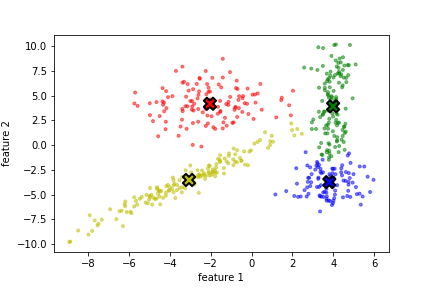
\includegraphics[width=0.6\textwidth]{figures/viterbi_2d.png}

\caption{Representation of the training data and the cluster means with state assigned by the Viterbi algorithm.}
\label{fig:viterbi_2d}
\end{center}
\end{figure}


\item %9

For the datapoints in the test set, we can compute the marginal probability $p(z_t|x_1,\dots,x_T)$ for each point to be in state $\{1,2,3,4\}$ for the parameters learned on the training set, similarly to question 2, where the parameters were given. Figure \ref{fig:real_parameters_inference} presents the probability of being in one of the four states as a function of time ($t$) for the first 100 points of the test set.

\begin{figure}[h!tbp]
\begin{center}
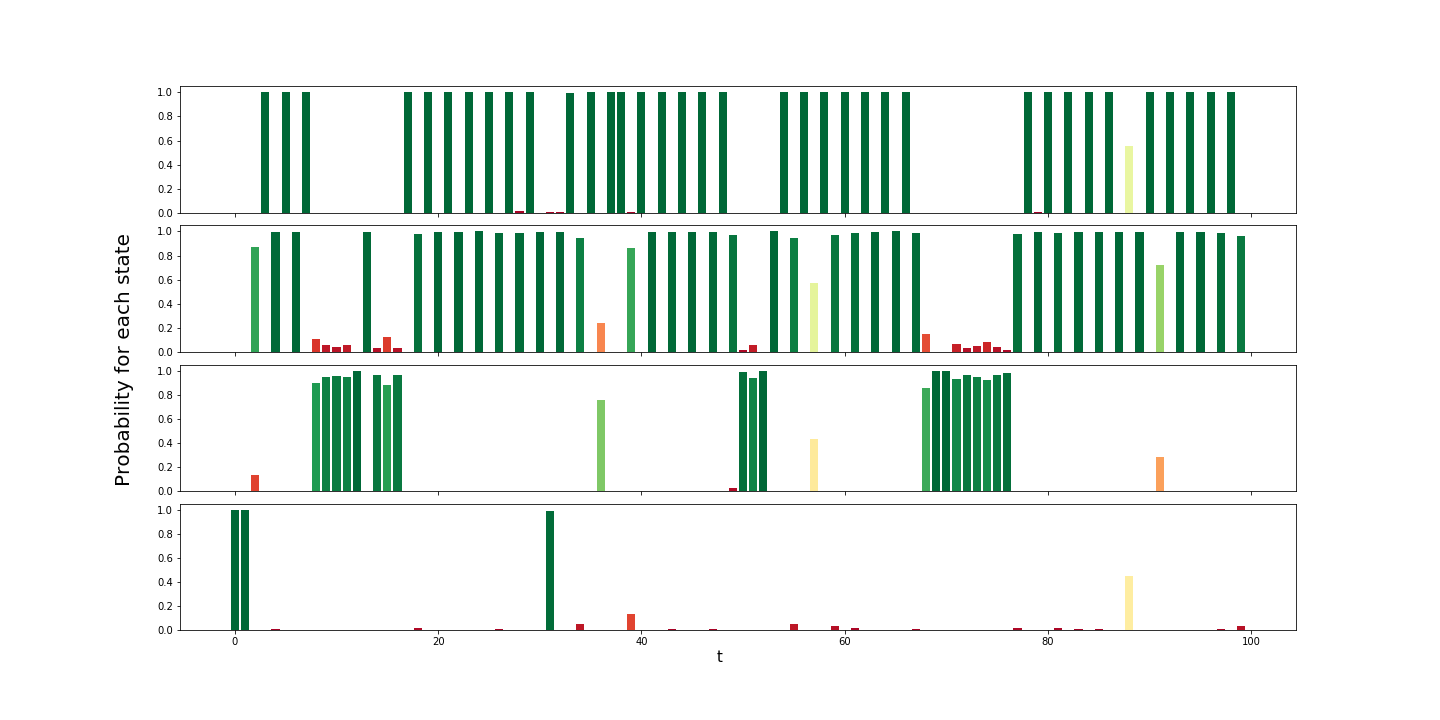
\includegraphics[width=\textwidth]{figures/real_param_inference.png}
\caption{Probability of the first 100 datapoints from the test set \texttt{EMGaussian.test} to be in state $\{1,2,3,4\}$ (top panel is state 1, bottom panel is state 4) as a function of time.}
\label{fig:real_parameters_inference}
\end{center}
\end{figure}

\clearpage

\item %10

For each of these same 100 points, figure \ref{fig:real_parameters_choice} presents the state where the marginal probability was the highest on figure \ref{fig:real_parameters_inference} as a function of time.

\begin{figure}[h!tbp]
\begin{center}
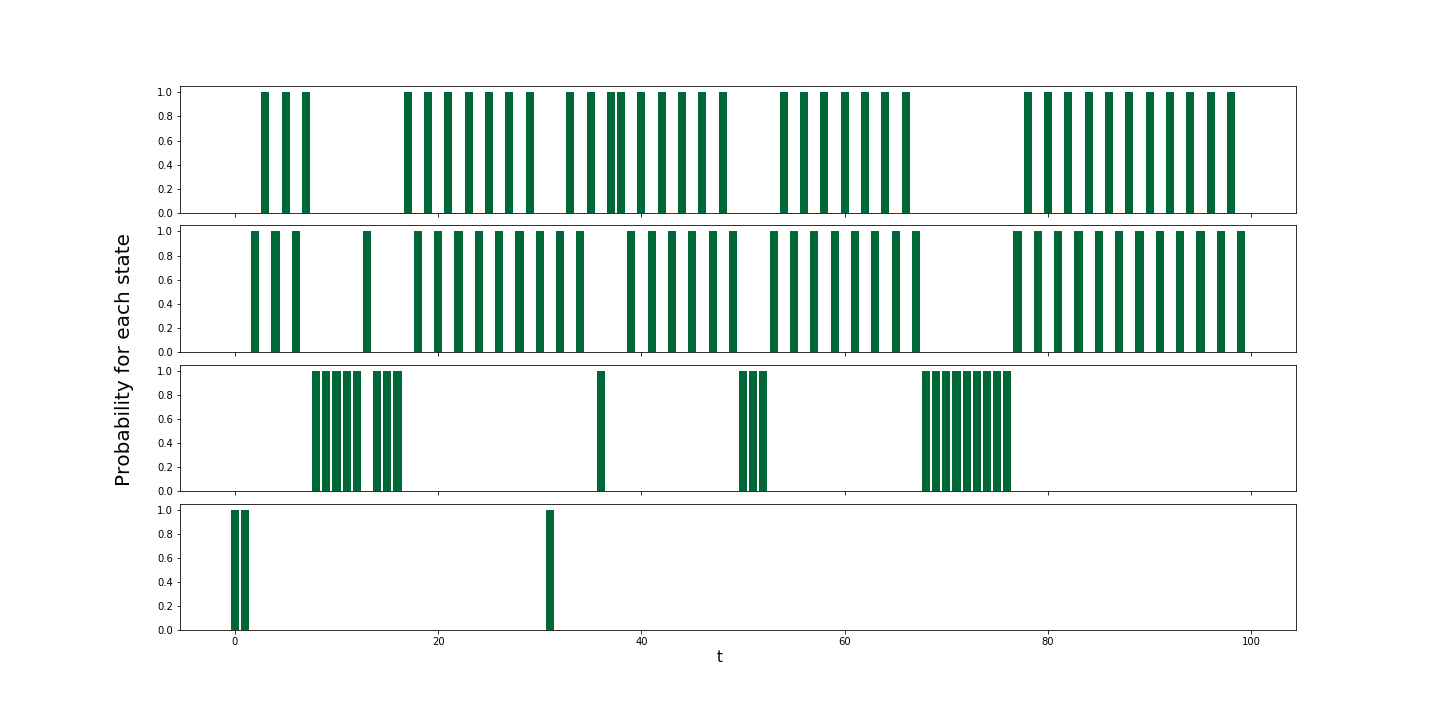
\includegraphics[width=0.9\textwidth]{figures/real_param_choice.png}
\caption{Most likely state of the first 100 datapoints from the test set \texttt{EMGaussian.test} (top panel is state 1, bottom panel is state 4) as a function of time.}
\label{fig:real_parameters_choice}
\end{center}
\end{figure}

\item %11

We can run the Viterbi algorithm on the test data to compare the most likely sequence of states obtained by the model with the sequence of states obtained at the previous question. Figure \ref{fig:real_parameters_viterbi} presents the most likely sequence of states for the first 100 points of the test set.

\begin{figure}[h!tbp]
\begin{center}
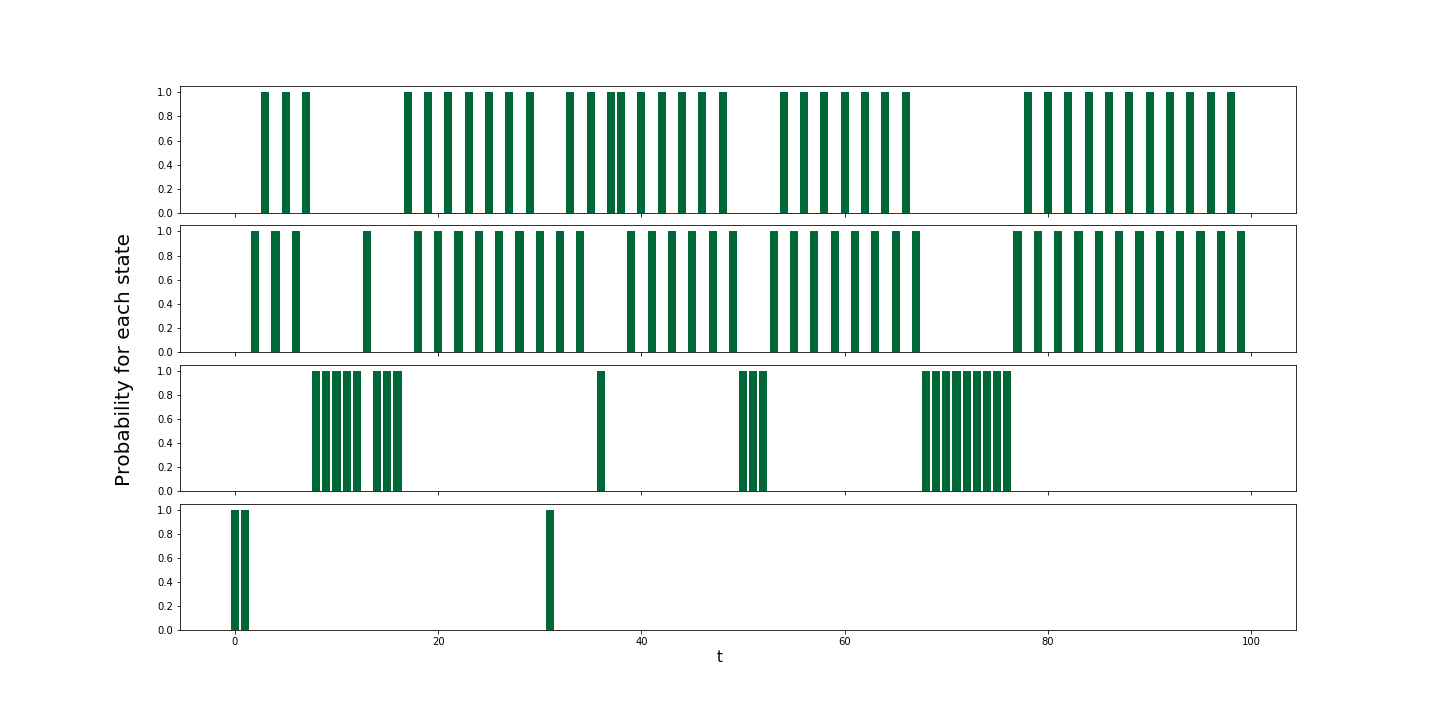
\includegraphics[width=0.9\textwidth]{figures/real_param_viterbi.png}
\caption{Most likely sequence of states of the first 100 datapoints from the test set \texttt{EMGaussian.test}  (top panel is state 1, bottom panel is state 4) using the Viterbi algorithm as a function of time.}
\label{fig:real_parameters_viterbi}
\end{center}
\end{figure}

We notice that the most likely sequence of states obtained with the Viterbi algorithm is exactly the same as the sequence of states obtained in question 10. This means that the data from the training set and the test set really depend on time and is not IID, as we postulated in the last homework. We thus have successfully trained our HMM!


\item %12

When the number of states $K$ is not known, we can set $K$ as an hyperparameter. Using three different datasets (a training set, a validation set and a test set), we can try different values of K and choose the value that yields the best results on sets that were not used for the training. We do so to ensure that our model can generalize well to new data. We can select the number of classes by trying them all, starting with 1, then 2, etc. or we can use a random search, trying different values randomly in a given range.


\end{enumerate}


\end{document}
